\section{Tuần 1}

\subsection{Giới thiệu đề tài}

\hspace{0.5cm} Trong giai đoạn 1 (Phase 1), nhóm đã xây dựng thuật toán tính toán tọa độ mục tiêu ở trạng thái tĩnh. Cụ thể, hệ thống nhận đầu vào là vị trí GPS của người quan sát, góc ngắm (azimuth, elevation) đo từ IMU hoặc la bàn điện tử, và khoảng cách đo bằng laser rangefinder. Đầu ra là tọa độ địa lý (kinh độ, vĩ độ, cao độ) của mục tiêu. Thuật toán được chạy theo kiểu single-point: mỗi lần tính toán là một lần đọc cảm biến riêng biệt, không có sự liên kết giữa các lần đo về mặt thời gian.

Giai đoạn 2 mở rộng bài toán: mục tiêu không còn đứng yên mà có thể di chuyển. Hệ thống phải tính toán liên tục, cập nhật vị trí mục tiêu theo thời gian thực và hiển thị quá trình di chuyển trên bản đồ số. Yêu cầu này đòi hỏi xử lý dòng dữ liệu từ nhiều cảm biến đồng thời, kết hợp chúng và áp dụng các bộ lọc để ước lượng vị trí chính xác ngay cả khi tín hiệu bị nhiễu hoặc gián đoạn.

Kiến trúc hệ thống được mở rộng theo các hướng sau:
\begin{itemize}[label={}]
    \item (i) Tích hợp thêm cảm biến IMU để đo hướng và góc nghiêng.
    \item (ii) Áp dụng thuật toán lọc Kalman và alpha-beta để xử lý chuỗi thời gian.
    \item (iii) Xây dựng hệ thống truyền thông thời gian thực bằng WebSocket (kênh truyền dữ liệu hai chiều).
    \item (iv) Xây dựng giao diện bản đồ tương tác trên nền web.
\end{itemize}
\hspace{0.5cm} Hệ thống được thiết kế để triển khai trên Raspberry Pi nhằm xử lý tại thiết bị di động trước khi gửi lên máy chủ trung tâm. Phần này thuộc triển khai phần cứng và được kiểm chứng qua mô phỏng trong giai đoạn hiện tại.

\subsection{Phát biểu bài toán}

\hspace{0.5cm} Bài toán được phát biểu như sau: Cho một người quan sát mang thiết bị GNSS (GPS), cảm biến IMU, và máy đo khoảng cách laser. Người quan sát này hướng thiết bị về phía mục tiêu đang di chuyển. Tại mỗi thời điểm, hệ thống cần:

\begin{itemize}
    \item Xác định vị trí hiện tại của người quan sát (kinh độ, vĩ độ, cao độ) từ thiết bị GNSS.
    \item Đo góc ngắm azimuth (góc giữa hướng Bắc và hướng ngắm, tính theo chiều kim đồng hồ) và góc elevation (góc cao so với mặt phẳng ngang) từ cảm biến IMU.
    \item Đo khoảng cách thực tế từ người quan sát đến mục tiêu bằng laser rangefinder.
    \item Tính toán tọa độ 3D của mục tiêu trong hệ tọa độ WGS84.
    \item Cập nhật liên tục vị trí mục tiêu khi cả người quan sát và mục tiêu đều di chuyển.
    \item Hiển thị lộ trình di chuyển của mục tiêu trên bản đồ số.
\end{itemize}

Các ràng buộc chính của bài toán:

\begin{itemize}
    \item Thời gian xử lý phải đảm bảo tính thời gian thực (độ trễ nhỏ hơn 100 ms).
    \item Dữ liệu từ các cảm biến bị ảnh hưởng bởi nhiễu môi trường và sai số chế tạo.
    \item Tín hiệu GPS có thể bị mất trong nhà hoặc khu vực bị che chắn.
    \item Khoảng cách laser chỉ hoạt động trong tầm nhìn thẳng (LOS), bị giới hạn bởi tầm xa của thiết bị.
    \item Mục tiêu có thể di chuyển với tốc độ khác nhau tùy theo loại (người đi bộ, xe máy, drone).
\end{itemize}

\subsection{Tổng quan hệ thống}

\hspace{0.5cm} Hệ thống được đề xuất gồm bốn tầng chính:

\subsubsection{Tầng cảm biến (Sensor Layer)}

\hspace{0.5cm} Tầng này bao gồm ba loại cảm biến chính:
\begin{itemize}
    \item \textbf{GNSS/GPS}: Cung cấp tọa độ tuyệt đối của người quan sát. Tần số thường 1-10 Hz. Độ chính xác phụ thuộc vào số vệ tinh hữu dụng, chất lượng thiết bị, và điều kiện môi trường. Trong điều kiện tốt, GPS dân sự đạt độ chính xác 2-5 m.
    \item \textbf{IMU} (Inertial Measurement Unit): Đo góc hướng (azimuth), góc nghiêng (elevation, roll, pitch). Cảm biến này có tần số cao (100-1000 Hz) nhưng bị trôi (drift) theo thời gian. Cần kết hợp với GPS để hiệu chỉnh.
    \item \textbf{Laser rangefinder}: Đo khoảng cách trực tiếp đến mục tiêu. Độ chính xác cao (thường +/- 1-2 cm) nhưng bị giới hạn bởi tầm xa và yêu cầu tầm nhìn thẳng.
\end{itemize}

\subsubsection{Tầng xử lý nhúng (Embedded Layer)}

\hspace{0.5cm} Để có thể nhận và xử lý dữ liệu thực tế từ các thiết bị phần cứng, Raspberry Pi (hoặc vi điều khiển tương tự) đóng vai trò là bộ phận đọc cảm biến và xử lý sơ bộ. Raspberry Pi nhận dữ liệu từ các cảm biến qua giao tiếp \textbf{UART/I2C/SPI}, đóng gói thành định dạng JSON, và gửi lên máy chủ thông qua kênh truyền dữ liệu hai chiều. Lớp này cũng có thể thực hiện các phép tính sơ bộ như chuẩn hóa dữ liệu, lọc nhiễu đơn giản, và kiểm tra lỗi trước khi gửi đi.

\subsubsection{Tầng máy chủ (Server Layer)}

\hspace{0.5cm} Máy chủ được xây dựng bằng FastAPI (Python), cung cấp các API REST để quản lý phiên (session) và kênh truyền dữ liệu hai chiều để nhận dữ liệu cảm biến thời gian thực. Tầng này đảm nhiệm:
\begin{itemize}
    \item Tiếp nhận dữ liệu từ Raspberry Pi.
    \item Chuyển đổi tọa độ giữa các hệ quy chiếu (WGS84, ECEF, ENU).
    \item Tính toán tọa độ mục tiêu từ vector định hướng và khoảng cách.
    \item Áp dụng Kalman filter hoặc alpha-beta filter để ước lượng vị trí và tốc độ.
    \item Phát dữ liệu đã xử lý xuống giao diện qua kênh truyền dữ liệu hai chiều.
\end{itemize}

\subsubsection{Tầng giao diện (Frontend Layer)}

\hspace{0.5cm} Giao diện người dùng được xây dựng bằng React kết hợp với Vite, sử dụng thư viện Leaflet để hiển thị bản đồ. Các chức năng chính:
\begin{itemize}
    \item Hiển thị bản đồ nền OpenStreetMap với vị trí người quan sát và mục tiêu.
    \item Cập nhật vị trí mục tiêu theo thời gian thực.
    \item Hiển thị lộ trình di chuyển của mục tiêu.
    \item Hiển thị thông số đo lường gồm tọa độ, góc và khoảng cách.
    \item Điều khiển phiên: bắt đầu, dừng, cấu hình.
\end{itemize}

\subsection{Cơ sở lý thuyết mở rộng}

\hspace{0.5cm} Giai đoạn 1 đã trình bày các kiến thức nền tảng về GPS, tam giác cầu, các phép chiếu bản đồ và các thuật toán geodesic (Haversine, Vincenty, Karney). Giai đoạn 2 mở rộng thêm các khái niệm sau:

\subsubsection{Hệ tọa độ Body frame và chuyển đổi}

\hspace{0.5cm} Bên cạnh các hệ tọa độ WGS84, ECEF, ENU đã sử dụng, dự án cần thêm hệ tọa độ Body frame (hệ tọa độ gắn với thiết bị). Body frame có gốc tại trọng tâm của thiết bị, trục x hướng về phía trước, trục y hướng sang phải, trục z hướng xuống dưới. Đây là hệ quy chiếu tự nhiên để mô tả góc ngắm azimuth và elevation.

Chuyển đổi từ Body frame sang ENU được thực hiện bằng ma trận xoay được xây dựng từ các góc roll, pitch, yaw đo từ IMU:

\begin{equation}
R_{body}^{ENU} = R_z(\text{yaw}) \cdot R_y(\text{pitch}) \cdot R_x(\text{roll})
\end{equation}

\subsubsection{Kết hợp đa cảm biến (Sensor fusion)}

\hspace{0.5cm} Việc kết hợp dữ liệu từ nhiều cảm biến là điểm khác biệt chính so với giai đoạn 1:
\begin{itemize}
    \item GPS cho vị trí tuyệt đối nhưng tần số thấp (từ 1 đến 10 Hz) và dễ mất tín hiệu.
    \item IMU có tần số cao (từ 100 đến 1000 Hz) nhưng bị trôi (drift) theo thời gian.
    \item Laser cho khoảng cách chính xác nhưng yêu cầu tầm nhìn thẳng (LOS).
\end{itemize}

Kết hợp ba nguồn này cho phép ước lượng vị trí mục tiêu ngay cả khi một hoặc hai cảm biến suy giảm. Nếu GPS mất tín hiệu, hệ thống vẫn ước lượng từ IMU và laser cho đến khi GPS hoạt động trở lại.

\subsubsection{Kalman filter}

\hspace{0.5cm} Kalman filter là thuật toán ước lượng trạng thái kinh điển trong điều khiển và dẫn đường, do Rudolf Kalman công bố năm 1960. Thuật toán ước lượng trạng thái của hệ thống từ các đo lường nhiễu và mô hình động học. Trong bài toán bám mục tiêu, Kalman filter ước lượng vị trí và tốc độ của mục tiêu.

Minh họa bộ lọc bằng mô hình đơn giản nhất: mô hình vận tốc không đổi (Constant Velocity) trong không gian 2D (East-North):

\begin{equation}
\begin{aligned}
\mathbf{x}_{k} &= \begin{bmatrix} e_k & n_k & \dot{e}_k & \dot{n}_k \end{bmatrix}^T \\
\mathbf{F}_{2D} &= \begin{bmatrix}
1 & 0 & \Delta t & 0 \\
0 & 1 & 0 & \Delta t \\
0 & 0 & 1 & 0 \\
0 & 0 & 0 & 1
\end{bmatrix}
\end{aligned}
\end{equation}

Với mục tiêu drone cần theo dõi cả trục Up, vector trạng thái mở rộng thành 6 chiều $\begin{bmatrix} e & n & u & \dot{e} & \dot{n} & \dot{u} \end{bmatrix}^T$ và ma trận $\mathbf{F}$ mở rộng tương ứng thành $6\times 6$ (bộ lọc 3D).

\subsubsection{Alpha-beta filter}

\hspace{0.5cm} Alpha-beta filter (còn gọi là g-h filter) là phiên bản đơn giản hóa của Kalman filter, chỉ dùng hai tham số: alpha cho vị trí và beta cho vận tốc. Bộ lọc này phù hợp với các hệ thống có tài nguyên tính toán hạn chế và vẫn cho kết quả tốt với các mục tiêu di chuyển đều.

\begin{equation}
\begin{aligned}
x_{k}^{p} &= x_{k-1} + \Delta t \cdot \dot{x}_{k-1} \quad \text{(Dự báo)} \\
x_{k} &= x_{k}^{p} + \alpha (z_{k} - x_{k}^{p}) \quad \text{(Cập nhật vị trí)} \\
\dot{x}_{k} &= \dot{x}_{k-1} + \frac{\beta}{\Delta t} (z_{k} - x_{k}^{p}) \quad \text{(Cập nhật vận tốc)}
\end{aligned}
\end{equation}

\subsection{Sơ đồ use-case}

\hspace{0.5cm} Hình \ref{fig:usecase} mô tả sơ đồ use-case của hệ thống. Người quan sát có thể khởi tạo phiên bám, cấu hình tham số, xem lộ trình hoặc dừng phiên. Hệ thống tự động cập nhật dữ liệu cảm biến, tính toán tọa độ và hiển thị trên bản đồ. Khi mất tín hiệu, hệ thống đưa ra cảnh báo.

\begin{figure}[htbp]
\centering
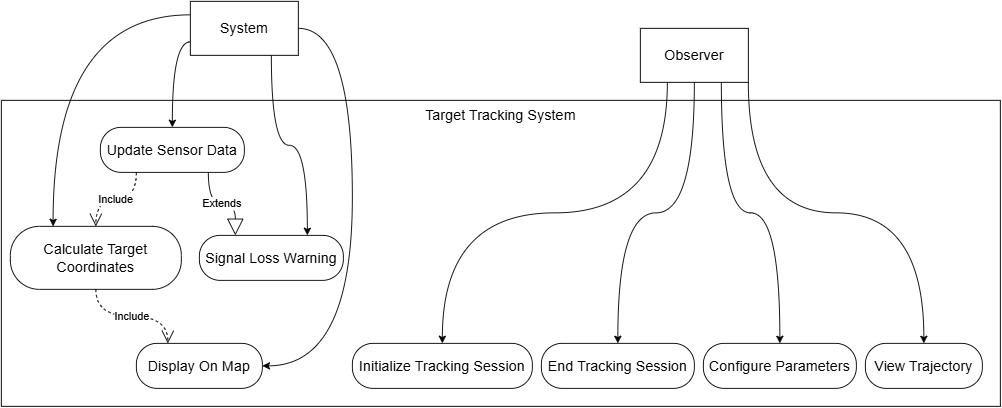
\includegraphics[width=0.7\textwidth]{Images/use-case-diagram.png}
\caption{Sơ đồ use-case của hệ thống tracking mục tiêu}
\label{fig:usecase}
\end{figure}
